\documentclass{report}

\input{~/dev/latex/template/preamble.tex}
\input{~/dev/latex/template/macros.tex}

\title{\Huge{}}
\author{\huge{Nathan Warner}}
\date{\huge{}}
\pagestyle{fancy}
\fancyhf{}
\lhead{Warner \thepage}
\rhead{}
% \lhead{\leftmark}
\cfoot{\thepage}
\setborder
% \usepackage[default]{sourcecodepro}
% \usepackage[T1]{fontenc}
\usepackage{pgfplots}
\pgfplotsset{compat=1.18}

\begin{document}
    % \maketitle
        \begin{titlepage}
       \begin{center}
           \vspace*{1cm}
    
           \textbf{Chapters 5-8}
    
           \vspace{0.5cm}
           Stat 128: Elementary Statistics
            
                
           \vspace{1.5cm}
   
           A Document By: \\
           \textbf{Nathan Warner}
    
           \vfill
                
                
           \vspace{0.8cm}
         
           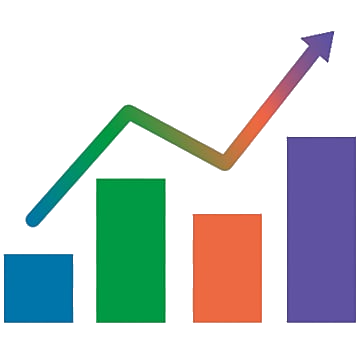
\includegraphics[width=0.4\textwidth]{../1-4/figures/2.png} \\
            July 03, 2023  \\
           Computer Science \\
           Joliet Junior College \\
           United States\\
           
                
       \end{center}
    \end{titlepage}
    \tableofcontents
    \pagebreak \bigbreak \noindent
    \section{Chapter 5}
    \bigbreak \noindent 
    \subsection{5.1: Probability Rules}
    \bigbreak \noindent 
    \textbf{\textit{\underline{Learning Objectives For This Section:}}}
    \begin{enumerate}
        \item \textbf{Understand Random Processes and the Law of Large Numbers}
        \item \textbf{Apply the Rules of Probabilities}
        \item \textbf{Compute and Interpret Probabilities Using the Empirical Method}
        \item \textbf{Compute and Interpret Probabilities Using the Classical Method}
        \item \textbf{Recognize and Interpret Subjective Probabilities}
    \end{enumerate}
    \bigbreak \noindent 
    \textbf{Vocab:}
    \begin{itemize}
        \item \textbf{Probability:} Is the measure of the likelihood of a random phenomenon or chance behavior occurring. It deals with experiments that yield random short-term results or outcomes yet reveal long-term predictability. The long-term proportion in which a certain outcome is observed is the probability of that outcome. 
        \item \textbf{Outcomes:} Short term results
        \item \textbf{The Law of Large Numbers:} As the number of repetitions of a probability experiment increases, the proportion with which a certain outcome is observed gets closer to the probability of the outcome.
        \item \textbf{an experiment} is any process with uncertain results that can be repeated.
        \item \textbf{The sample space, $S$,} of a probability experiment is the collection of all possible outcomes for that experiment.
        \item \textbf{An event} is any collection of outcomes from a probability experiment. An event consists of one or more outcomes. We denote events with one outcome, sometimes called simple events, as $e_{i}$. In general, events are denoted using capital letters such as $ E$.
        \item \textbf{A probability model} lists the possible outcomes of a probability experiment and each outcome's probability. A probability model must satisfy Rules 1 and 2 of the rules of probabilities.
        \item  \textbf{An unusual event} is an event that has a low probability of occurring.
        \item An experiment has \textbf{equally likely outcomes} when each outcome has the same probability of occurring. 
        \item A \textbf{subjective probability} is a probability that is determined based on personal judgment.








    \end{itemize}

\end{document}
